\chapter{Conception fonctionnelle et technique}

\textbf{IMPORTANT :} Cette phase de conception est \textbf{CRUCIALE} et a été \textbf{COMPLÈTEMENT TERMINÉE} avant le démarrage du développement. Pour \textbf{App Budget V3}, j'ai construit une conception fonctionnelle et technique détaillée, validée itérativement, qui sert de référence unique au développement, aux tests et à la soutenance.

\section{Méthodologie de conception}

La conception d'\textbf{App Budget V3} s'est déroulée en plusieurs étapes structurées :

\begin{enumerate}
    \item \textbf{Cadrage fonctionnel :} Identification des besoins critiques à partir des personae.
    \item \textbf{Modélisation des Use Cases :} Liste et priorisation des cas d'usage (MoSCoW).
    \item \textbf{Diagrammes UML :} Cas d'utilisation, Classes et Séquences pour les flux critiques.
    \item \textbf{Conception UI/UX :} Zoning, Wireframes et Maquettes Figma haute fidélité.
    \item \textbf{Modélisation des données :} MCD $\rightarrow$ MLD $\rightarrow$ MPD (PostgreSQL).
    \item \textbf{Architecture 3-tiers :} Formalisation de la stack Next.js / NestJS / PostgreSQL.
    \item \textbf{Plan de tests :} Définition des critères d'acceptation par User Story.
    \item \textbf{Validation :} Relecture globale avant implémentation.
\end{enumerate}

\begin{conseil}
\textbf{Pourquoi la conception est-elle stratégique ?}
\begin{itemize}
    \item \textbf{Évite les refactorisations :} Le modèle de données a été figé avant le code.
    \item \textbf{Guide le développement :} 1 User Story = 1 Use Case + 1 Séquence + 1 Maquette.
    \item \textbf{Facilite les tests :} Les flux UML servent de base aux scénarios E2E Playwright.
    \item \textbf{Réduit les risques :} Anticipation des cas d'erreurs (CSV invalide, Auth failed).
\end{itemize}

\textbf{Checklist de validation :}
\begin{itemize}
    \item[\mycheckmark] Diagrammes de cas d'usage (Use Cases) validés
    \item[\mycheckmark] Diagramme de classes UML complet
    \item[\mycheckmark] Diagrammes de séquence critiques (Auth, Transaction, Import)
    \item[\mycheckmark] Modèle de données PostgreSQL défini
    \item[\mycheckmark] Architecture technique Dockerisée validée
    \item[\mycheckmark] Maquettes Figma (Desktop + Mobile) terminées
    \item[\mycheckmark] Plan de tests (Unitaires, E2E) établi
\end{itemize}
\end{conseil}

% ============================================================
% USE CASES
% ============================================================

\section{Modélisation fonctionnelle (UML)}

\subsection{Acteurs et Cas d'Usage}

Les interactions du système sont définies par trois acteurs principaux :
\begin{itemize}
    \item \textbf{Utilisateur authentifié :} Suit son budget (Léa, Marc).
    \item \textbf{Administrateur :} Monitore l'application et les statistiques globales.
    \item \textbf{Système externe :} Service d'envoi d'emails et notifications.
\end{itemize}

\textbf{Principaux cas d'usage (UC) :}
\begin{itemize}
    \item \textbf{UC01 -- Compte :} Inscription, connexion, gestion profil.
    \item \textbf{UC02 -- Transactions :} CRUD complet, filtres (Revenus/Dépenses).
    \item \textbf{UC03 -- Enveloppes :} Définition des plafonds, suivi consommation.
    \item \textbf{UC04 -- Dashboard :} Visualisation des KPIs et graphiques.
    \item \textbf{UC05 -- Import :} Traitement fichiers CSV bancaires.
    \item \textbf{UC06 -- Export :} Portabilité des données (RGPD).
\end{itemize}

\begin{figure}[H]
    \centering
    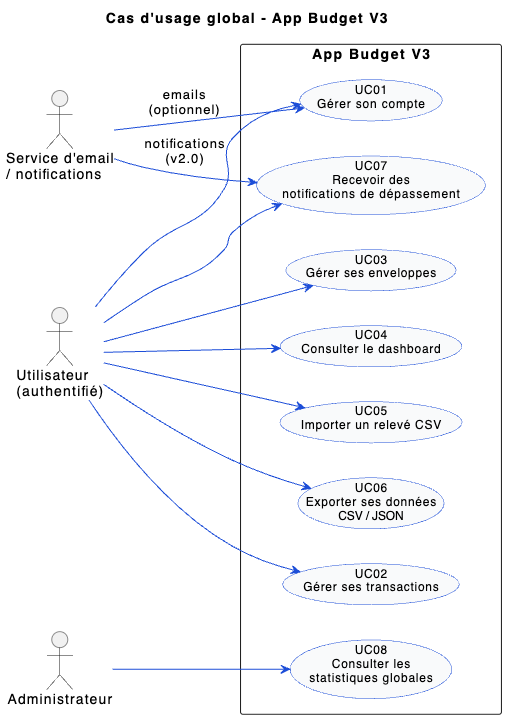
\includegraphics[width=0.95\textwidth]{assets/images/usage_global.png}
    \caption{Diagramme de cas d'usage global -- App Budget V3}
    \label{fig:usage_global}
\end{figure}

\begin{jury}
\textbf{Points de vigilance contrôlés :}
\begin{itemize}
    \item Les cas d'usage critiques sont tous traçables vers des User Stories.
    \item Les flux alternatifs (erreurs) sont documentés dans les critères d'acceptation.
    \item La distinction des rôles (User vs Admin) est claire.
\end{itemize}
\end{jury}

% ============================================================
% DIAGRAMME DE CLASSES
% ============================================================

\section{Modélisation statique : Diagramme de Classes}

Ce diagramme structure les données manipulées par l'application et sert de référence pour le développement Back-end (NestJS) et la base de données.

\begin{figure}[H]
    \centering
    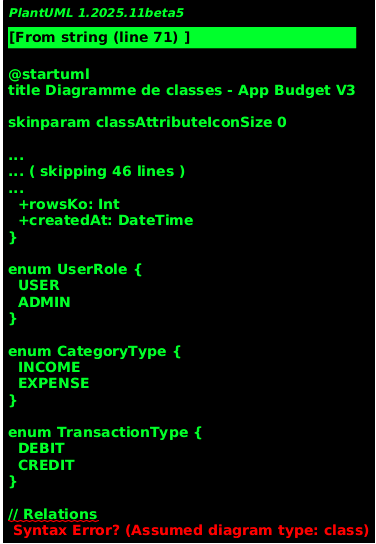
\includegraphics[width=0.95\textwidth]{assets/images/class-diagram-app-budget-v3.png}
    \caption{Diagramme de classes UML détaillé}
    \label{fig:class-diagram}
\end{figure}

\begin{tcolorbox}[colback=blue!5!white,colframe=blue!60!black,title=\textbf{Mapping UML $\leftrightarrow$ Prisma (Code)}]
Chaque classe UML est traduite en modèle Prisma pour assurer la cohérence :

\begin{lstlisting}[language=JavaScript]
// Classe UML User -> Modele Prisma
model User {
  id           Int       @id @default(autoincrement())
  email        String    @unique
  passwordHash String
  role         UserRole  @default(USER)
  currency     String    @default("EUR")
  
  // Relations definies dans le diagramme
  transactions Transaction[]
  envelopes    BudgetEnvelope[]
}
\end{lstlisting}
\end{tcolorbox}

% ============================================================
% DIAGRAMMES DE SEQUENCE
% ============================================================

\section{Modélisation dynamique : Diagrammes de Séquence}

Les séquences détaillent les interactions temporelles entre le Frontend, l'API et la Base de données.

\subsection{Séquence 1 : Authentification (US-01)}

\begin{figure}[H]
    \centering
    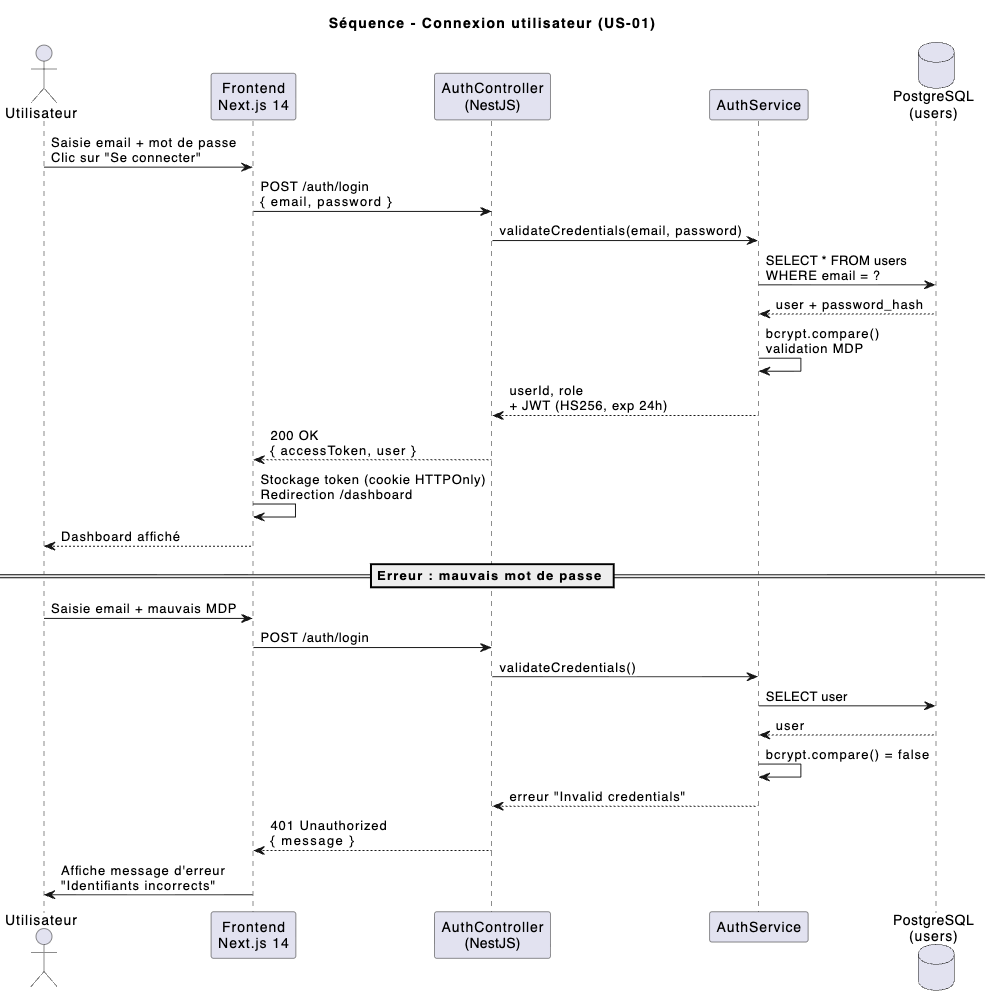
\includegraphics[width=0.95\textwidth]{assets/images/seq-auth-login.png}
    \caption{Flux de connexion utilisateur (Login)}
    \label{fig:seq-auth}
\end{figure}

\textbf{Déroulement nominal :}
\begin{enumerate}
    \item Saisie des identifiants sur le Frontend (Next.js).
    \item Appel API \texttt{POST /auth/login}.
    \item Le Backend vérifie le hash du mot de passe (bcrypt).
    \item Génération d'un token JWT (signé HS256).
    \item Retour \texttt{200 OK} et redirection vers le Dashboard.
\end{enumerate}

\subsection{Séquence 2 : Création de Transaction (US-03)}

\begin{figure}[H]
    \centering
    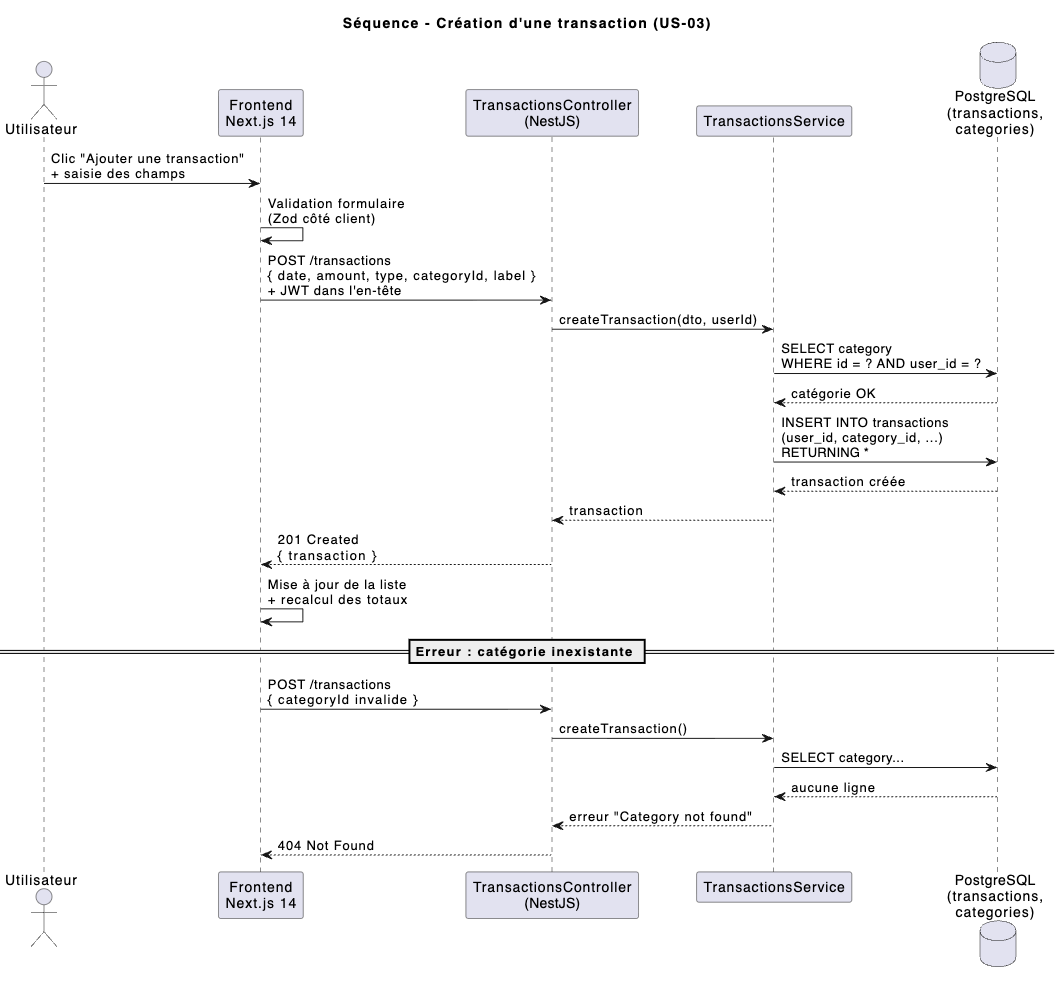
\includegraphics[width=0.95\textwidth]{assets/images/seq-create-transaction.png}
    \caption{Flux de création d'une transaction}
    \label{fig:seq-transaction}
\end{figure}

Ce diagramme illustre la validation des données par le \texttt{TransactionsService} avant l'insertion en base via Prisma, garantissant l'intégrité des données financières.

\subsection{Séquence 3 : Alertes Budgétaires (US-07)}

\begin{figure}[H]
    \centering
    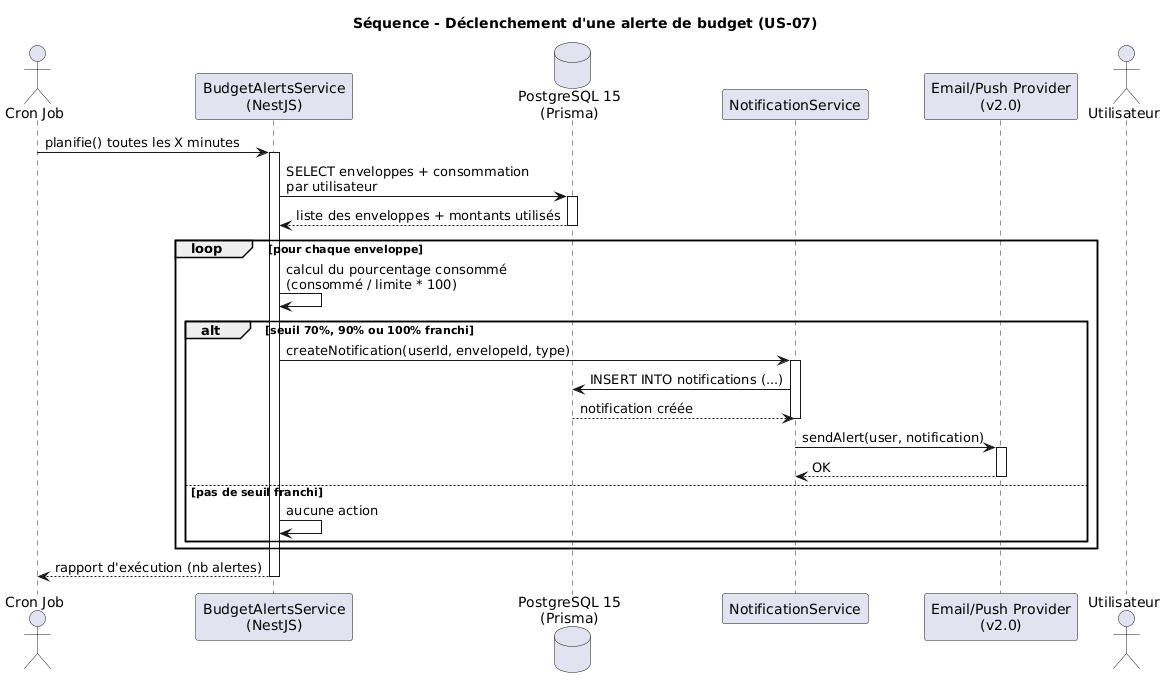
\includegraphics[width=0.95\textwidth]{assets/images/seq-budget-alert.png}
    \caption{Flux automatique de déclenchement d'alertes}
    \label{fig:seq-alert}
\end{figure}

% ============================================================
% UI / UX
% ============================================================

\section{Conception de l'Interface (UI/UX)}

La conception graphique a suivi une approche \textbf{"Mobile First"}, validée en trois étapes : Zoning, Wireframes, Maquettes.

\subsection{Zoning et Structure}

Exemple de structuration de la page \textbf{Dashboard} :

\begin{center}
\small
\begin{tabular}{|p{0.3\textwidth}|p{0.6\textwidth}|}
\hline
\multicolumn{2}{|c|}{\textbf{Header (Logo, Navigation, Profil)}} \\
\hline
\textbf{Latéral (Mobile: Menu)} & \textbf{Zone Centrale (Contenu)} \\
\hline
- Navigation & - \textbf{KPIs} : Revenus, Dépenses, Reste à vivre \\
- Filtres dates & - \textbf{Graph 1} : Évolution mensuelle (Courbe) \\
- Bouton "Ajouter" & - \textbf{Graph 2} : Répartition par catégorie (Pie) \\
\hline
\multicolumn{2}{|c|}{\textbf{Footer (Mentions, RGPD)}} \\
\hline
\end{tabular}
\end{center}

\subsection{Wireframes et Maquettes (Figma)}

\begin{figure}[H]
    \centering
    \begin{minipage}{0.45\textwidth}
        \centering
        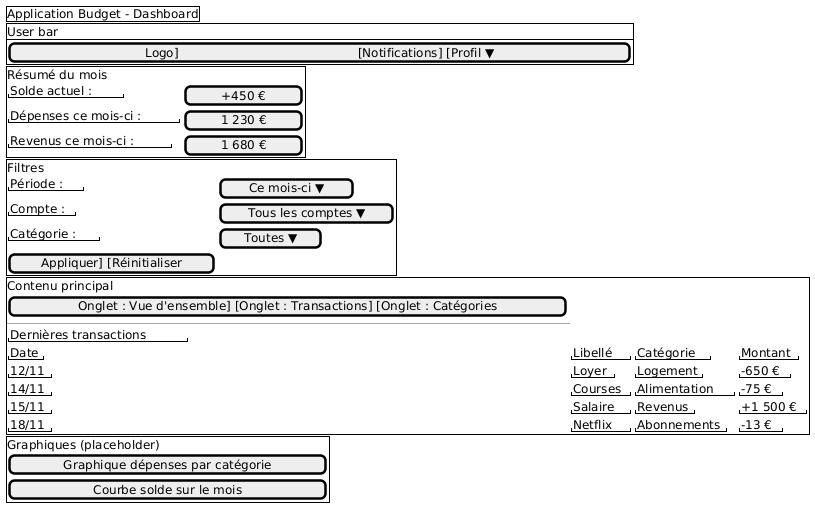
\includegraphics[width=\textwidth]{assets/images/wireframe-dashboard.png}
        \caption{Wireframe Basse Fidélité}
    \end{minipage}\hfill
    \begin{minipage}{0.45\textwidth}
        \centering
        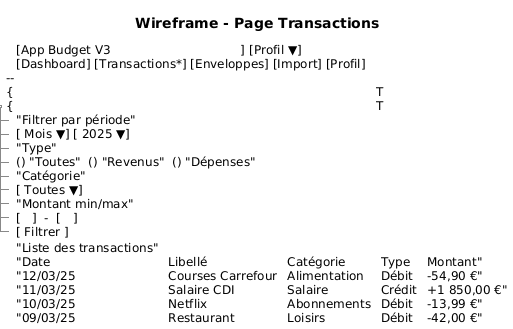
\includegraphics[width=\textwidth]{assets/images/wireframe-transactions.png}
        \caption{Wireframe Transactions}
    \end{minipage}
\end{figure}

Les maquettes Haute Fidélité intègrent la charte graphique finale, les interactions (hover, focus) et les composants réutilisables du Design System.

\subsection{Charte Graphique (Design System)}

\begin{center}
\small
\begin{tabular}{|p{0.25\textwidth}|p{0.2\textwidth}|p{0.45\textwidth}|}
\hline
\textbf{Élément} & \textbf{Valeur} & \textbf{Usage} \\
\hline
\textbf{Bleu Primaire} & \texttt{\#1D4ED8} & Actions principales, Header \\
\hline
\textbf{Vert Succès} & \texttt{\#22C55E} & Revenus, Soldes positifs \\
\hline
\textbf{Orange Alerte} & \texttt{\#F97316} & Warning (Budget > 80\%) \\
\hline
\textbf{Rouge Danger} & \texttt{\#EF4444} & Erreurs, Dépenses, Dépassements \\
\hline
\textbf{Typographie} & \textit{Inter} & Police sans-serif moderne et lisible \\
\hline
\end{tabular}
\end{center}

% ============================================================
% BASE DE DONNÉES
% ============================================================

\section{Conception de la Base de Données (PostgreSQL)}

Le modèle de données a été conçu selon la méthode Merise (MCD/MLD/MPD) puis implémenté physiquement sous PostgreSQL 15.

\subsection{Modèle Conceptuel (MCD)}

\begin{figure}[H]
    \centering
    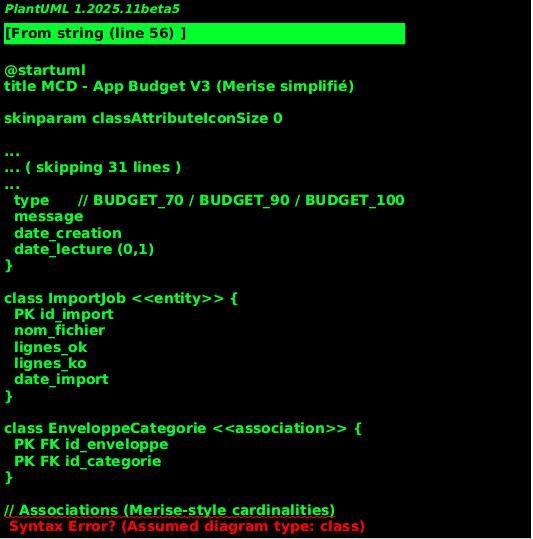
\includegraphics[width=0.95\textwidth]{assets/images/mcd-app-budget-v3.png}
    \caption{MCD : Entités et relations}
    \label{fig:mcd}
\end{figure}

\subsection{Implémentation Physique (SQL)}

Extrait du script de création des tables (généré et géré par Prisma Migrate) :

\begin{lstlisting}[language=SQL]
-- Table des transactions avec contraintes
CREATE TABLE transactions (
  id SERIAL PRIMARY KEY,
  user_id INTEGER NOT NULL REFERENCES users(id) ON DELETE CASCADE,
  category_id INTEGER NOT NULL REFERENCES categories(id),
  date DATE NOT NULL,
  amount NUMERIC(12,2) NOT NULL,
  type TEXT NOT NULL CHECK (type IN ('DEBIT','CREDIT')),
  label TEXT NOT NULL,
  created_at TIMESTAMPTZ DEFAULT NOW()
);

-- Index de performance pour le Dashboard
CREATE INDEX idx_transactions_user_date ON transactions(user_id, date DESC);
\end{lstlisting}

% ============================================================
% ARCHITECTURE
% ============================================================

\section{Architecture Technique 3-Tiers}

L'application repose sur une séparation stricte des responsabilités.

\begin{figure}[H]
    \centering
    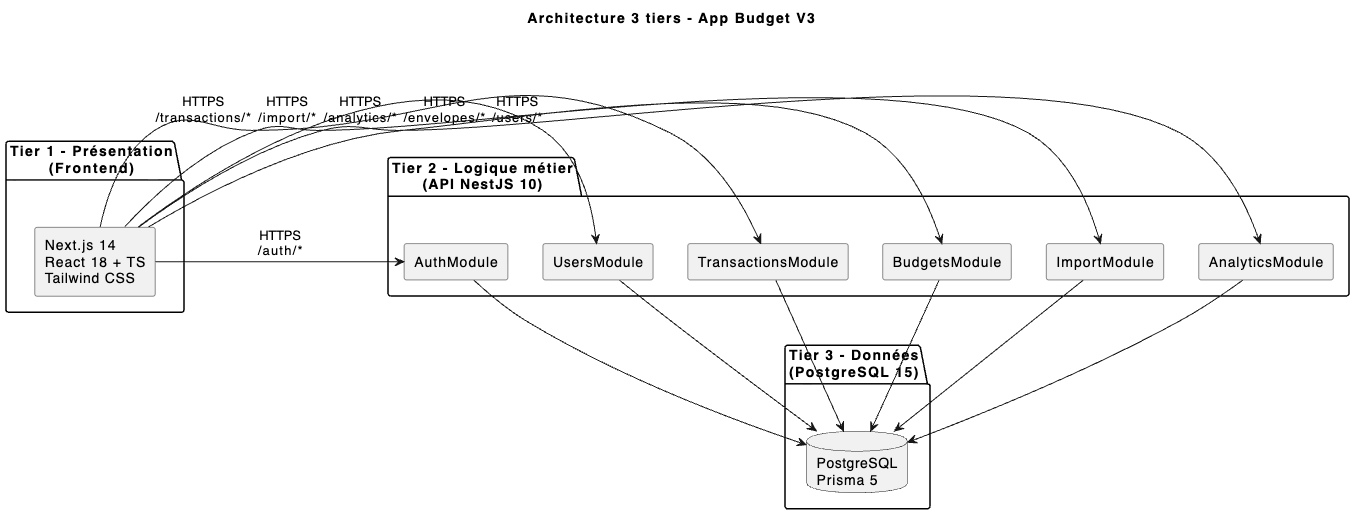
\includegraphics[width=0.9\textwidth]{assets/images/arch-3tiers-app-budget-v3.png}
    \caption{Architecture : Next.js (Front) - NestJS (Back) - PostgreSQL (Data)}
    \label{fig:arch-3tiers}
\end{figure}

\begin{itemize}
    \item \textbf{Tier 1 (Présentation) :} \textbf{Next.js 14}. Rendu hybride (SSR/CSR), composants React, validation formulaires (Zod).
    \item \textbf{Tier 2 (Métier) :} \textbf{NestJS 10}. API RESTful, Auth Guards, Services métier, Validation DTO.
    \item \textbf{Tier 3 (Données) :} \textbf{PostgreSQL 15}. Base relationnelle robuste, intégrité référentielle, gérée via Prisma ORM.
\end{itemize}

\section{Matrice de Cohérence Globale}

Le tableau ci-dessous démontre la traçabilité complète du besoin jusqu'au code :

\begin{center}
\small
\begin{tabular}{|p{0.15\textwidth}|p{0.15\textwidth}|p{0.2\textwidth}|p{0.2\textwidth}|p{0.15\textwidth}|}
\hline
\textbf{Use Case} & \textbf{Classe UML} & \textbf{Endpoint API} & \textbf{Table SQL} & \textbf{Écran UI} \\
\hline
UC01 Auth & User & \texttt{POST /auth/login} & \texttt{users} & Login \\
\hline
UC02 Transac. & Transaction & \texttt{POST /transactions} & \texttt{transactions} & Formulaire \\
\hline
UC03 Budget & BudgetEnv. & \texttt{GET /budgets} & \texttt{budget\_envelopes} & Liste env. \\
\hline
UC04 Dash. & (Agregats) & \texttt{GET /analytics} & (Join queries) & Dashboard \\
\hline
UC05 Import & ImportJob & \texttt{POST /import} & \texttt{import\_jobs} & Upload \\
\hline
\end{tabular}
\end{center}

\begin{tcolorbox}[colback=green!5!white,colframe=green!60!black,title=\textbf{Exemple de traçabilité : UC02 Transactions}]
\textbf{Besoin :} US-03 "Créer une transaction" \\
$\rightarrow$ \textbf{UML :} Classe \texttt{Transaction}, Séquence \texttt{CreateTransaction} \\
$\rightarrow$ \textbf{API :} \texttt{TransactionsController.create()} \\
$\rightarrow$ \textbf{DB :} Table \texttt{transactions} (FK user\_id, category\_id) \\
$\rightarrow$ \textbf{UI :} Page \texttt{/transactions/new}
\end{tcolorbox}

\section{Ressources et Références}

\begin{itemize}
    \item \textbf{UML \& Merise :} \url{https://www.uml-diagrams.org/}
    \item \textbf{Frameworks :} \url{https://nextjs.org/} (Front), \url{https://nestjs.com/} (Back)
    \item \textbf{Base de données :} \url{https://www.postgresql.org/docs/}
    \item \textbf{Outils :} Figma (UI), Draw.io (Diagrammes)
\end{itemize}